\documentclass{standalone}
\usepackage{chez}

\begin{document}
%\chapter{November 26, 2019}

\section{Oracles}
\begin{definition}
  Given a language \(A\), an \vocab{\(A\)-oracle machine} (\(A\)-\textsf{OM}) is a \textsf{TM} that magically knows the answer to \(A\).
\end{definition}
One way to formalize this is to add two extra tapes to our regular \textsf{TM}s. One request tape and one answer tape. When we change the request tape, the answer tape changes to the answer of the instance on the request tape immediately, and we can then read from it.

Even though we can never have oracles in real life, we study oracles because if we can show that we can't solve a problem even with an oracle, then we know the problem is really hard.

\begin{definition}
  Let \(\mathsf{P}^{A}\) be the class of languages solvable in polynomial time by an \textit{A}-\textsf{OM}. If \(L \in \mathsf{P}^{A}\), then we say that we can solve \(L\) in polynomial time relative to \textit{SAT}. We can similarly define \(\mathsf{NP}^{A}\).
\end{definition}

\begin{example}
  A \textit{SAT}-\textsf{OM} can solve \textit{SAT}. In particular, we can copy the input into the request tape, and then accept or reject according to the response we get on the answer tape.
\end{example}

Note that this means that
\[
  \mathsf{NP} \subseteq \mathsf{P}^{\textit{SAT}}.
\]
Having an oracle feels like performing reductions, but it is more powerful. In particular, we can request multiple instances of a problem. Moreover, we know that \(\mathsf{P}^{\textit{SAT}} = \mathsf{co}(\mathsf{P}^{\textit{SAT}}) = \mathsf{coP}^{\textit{SAT}}\) because we are working with determinism, so we also have \(\mathsf{NP} \subseteq \mathsf{coP}^{\textit{SAT}} \implies \mathsf{coNP} \subseteq \mathsf{P}^{\textit{SAT}}\).

\begin{example}
  Let \(\textit{MINFORM} = \set{\angles \phi \mid \text{$\phi$ is a minimal formula}}\). We claim \(\textit{MINFORM} \in \mathsf{coNP}^{\textit{SAT}}\).
  \tcblower
  The idea is to nondeterministically guess a shorter formula \(\varphi\), and then use the oracle to check whether they are equivalent by writing the formula \((\phi \Rightarrow \varphi) \land (\varphi \Rightarrow \phi)\).
\end{example}

\subsection{Limits on Diagonalization}
It turns out that the problem of whether \(\mathsf{P}^{\textit{SAT}} \overset{?}{=} \mathsf{NP}^{\textit{SAT}}\) is open. However, we have the following surprising fact:

\begin{proposition}
  \(\mathsf{P}^{\textit{TQBF}} = \mathsf{NP}^{\textit{TQBF}} \subseteq \mathsf{NPSPACE}\).
\end{proposition}
\begin{proof}
  We know that \(\mathsf{P}^{\mathit{TQBF}} \subseteq \mathsf{NP}^{\mathit{TQBF}}\). Since \(\textit{TQBF}\) is \(\textsf{PSPACE}\)-complete, we have \(\textsf{PSPACE} \subseteq \mathsf{P}^{\textit{TQBF}}\). Therefore, we have the chain of inclusions
  \[
    \mathsf{NP}^{\textit{TQBF}} \subseteq
    \mathsf{NPSPACE} = \mathsf{PSPACE} \subseteq \mathsf{P}^{\textit{TQBF}},
  \]
  where the first inclusion is from the fact that \(\textit{TQBF} \in \mathsf{NPSPACE}\), so an \(\mathsf{NPSPACE}\) machine can just solve \textit{TQBF} itself instead of asking the oracle. Therefore, \(\mathsf P^{\textit{TQBF}} = \mathsf{NP}^{\mathit{TQBF}}\).
\end{proof}

Note that if we can use a diagonalization argument to show that \(\mathsf{P} \neq \mathsf{NP}\), then we can just use the same argument to show that \(\mathsf{P}^{\textit{A}} \neq \mathsf{NP}^{\textit{A}}\). However, this is a contradiction for \(A = \textit{TQBF}\), so we cannot use a pure diagonalization argument to prove \(\mathsf{P} \neq \mathsf{NP}\).

\begin{question}
  Recall that \(A_{\textsf{TM}}\) is undecidable from diagonalization. Why doesn't this rule out the existence of \(A_{\textsf{TM}}\)-\textsf{OM}s?
  \tcblower
  Diagonalization only states that \(A_{\textsf{TM}}\) is undecidable by regular \textsf{TM}s, and that \(A_{\textsf{$L$-OM}}\) is undecidable by \(L\)-\textsf{OM}s.
\end{question}



\subsection{More Oracle Problems}
Suppose we have two friends (but not that good of friends that they trust each other) Al and Bo (short for Alice and Bob) that want to split cake fairly.

The protocol goes as follows. There is a cake and several predetermined cuts. Al selects a subset of the cuts, and the cake is cut along those curves. If this process produces \(n\) pieces of cake, Bo then selects \(\ceil{n/2}\) pieces.

\begin{example}
  If this was the original cake with predetermined cuts, Al can select all the cuts, and Bo must select two pieces, guaranteed to have equal area, so Al can guarantee fair cuts.

  \begin{center}
    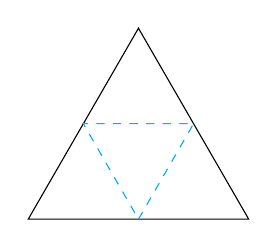
\begin{tikzpicture}[scale=0.7]
      \draw (0, 0) -- +(0: 4) -- +(60: 4) -- cycle;
      \draw[dashed, cyan] (2, 0) -- +(60: 2) -- +(120: 2) -- cycle;
    \end{tikzpicture}
  \end{center}
\end{example}

Let the problem be
\[
  \textit{CAKE} = \set{
    (\text{cakes}, \text{allowed cuts}) \mid \text{Al can guarantee fair cuts}
  }
\]

\begin{proposition}
  \(\textit{CAKE} \in \mathsf{NP}^{\textit{UNSAT}}\), i.e.\ using an \textsf{NTM} with an \(\textit{UNSAT}\) oracle, we can solve \(\textit{CAKE}\).
\end{proposition}
\begin{proof}
  Consider the following algorithm. Let the \textsf{NTM} nondeterministically select the subset of cuts that Al chooses. We have some pieces of cake with certain volumes. Consider the formula that says ``the volumes of the partition are unequal'', where the variables are indicator variables of whether a piece is in the partition. Then, use the oracle to determine whether this formula is unsatisfiable. If so, then any choice Bo will make must be fair.
\end{proof}

\begin{example}
  Consider the problem
  \[
    \textit{GETSAT} = \set{
      \angles{\phi, i, b} \mid \text{$\phi$ is satisfiable where in the minimal satisfying assignment, the $i$th variable is $b$}
    }.
  \]
  Then \(\textit{GETSAT} \in \mathsf{P}^{\textit{SAT}}\) because we can substitute in \(b\) for the \(i\)th variable of \(\phi\), and then ask the oracle whether the new formula is satisfiable.
\end{example}


\section{Probabilistic Turing Machines}
\begin{definition}
  Let a \vocab{probabilistic Turing machine} (\textsf{PTM}) be a decider \textsf{NTM} where at each nondeterministic step, there are two options, and there is a \(\half\) probability of choose each option.
\end{definition}

For each branch, we can consider the probability that the machine has taken it, i.e.\ \(2^{-k}\), where \(k\) is the number of nondeterministic states in that branch. Then, we define
\[
  \PP[\text{$M$ accepts $w$}] \coloneqq \sum_{\substack{\text{accepting} \\ \mathclap{\text{branches $b$}}}} \PP[\text{$M$ takes branch $b$}],
\]
and \(\PP[\text{$M$ rejects $w$}] \coloneqq 1 - \PP[\text{$M$ accepts $w$}]\).

\begin{definition}
  For some \(\eps > 0\), we say that a \textsf{PTM} \(M\) decides \(A\) with error probability \(\eps\) if:
  \begin{itemize}
    \item for all \(w \in A\), \(\PP[\text{$M$ accepts $w$}] > 1 - \eps\) and
    \item for all \(w \notin A\), \(\PP[\text{$M$ rejects $w$}] > 1 - \eps\).
  \end{itemize}
\end{definition}

Then we can define a new complexity class.
\begin{definition}[Bounded Probabilistic Polynomial Time]
  Let \(\mathsf{BPP} = \set{A \mid \text{some polynomial time \textsf{PTM} decides $A$ with error probability $1/3$}}\).
\end{definition}

The \(\frac{1}{3}\) in the definition seems a bit strange. It turns out that the choice of the constant here does not matter!
\begin{proposition}[Amplification Lemma]
  For \(0 < \eps_1, \eps_2 < \half\), any \textsf{PTM} \(M_1\) with error probability \(\eps_1\) has an equivalent \textsf{PTM} \(M_2\) with error probability \(\eps_2\).
\end{proposition}
\begin{proof}[Sketch]
    \(M_2\) can just run \(M_1\) multiple times, and return the answer that appears the most often.
\end{proof}
Therefore, we have the equivalent definition
\[
  \mathsf{BPP} = \set*{A \mid \text{some polynomial time \textsf{PTM} decides $A$ with error probability $\eps < \half$}}.
\]



\end{document}

